\documentclass[
11pt, % The default document font size, options: 10pt, 11pt, 12pt
%oneside, % Two side (alternating margins) for binding by default, uncomment to switch to one side
english, % ngerman for German
singlespacing, % Single line spacing, alternatives: onehalfspacing or doublespacing
%draft, % Uncomment to enable draft mode (no pictures, no links, overfull hboxes indicated)
%nolistspacing, % If the document is onehalfspacing or doublespacing, uncomment this to set spacing in lists to single
%liststotoc, % Uncomment to add the list of figures/tables/etc to the table of contents
%toctotoc, % Uncomment to add the main table of contents to the table of contents
parskip, % Uncomment to add space between paragraphs
%nohyperref, % Uncomment to not load the hyperref package
headsepline, % Uncomment to get a line under the header
chapterinoneline, % Uncomment to place the chapter title next to the number on one line
%consistentlayout, % Uncomment to change the layout of the declaration, abstract and acknowledgements pages to match the default layout
]{MastersDoctoralThesis} % The class file specifying the document structure
\usepackage{url}
\usepackage[utf8]{inputenc} % Required for inputting international characters
\usepackage[T1]{fontenc} % Output font encoding for international characters
\usepackage{lipsum}
\usepackage{mathpazo} % Use the Palatino font by default
\usepackage{fltrace}
\usepackage[backend=bibtex,style=authoryear,natbib=true]{biblatex} % Use the bibtex backend with the authoryear citation style (which resembles APA)

\addbibresource{bibliography.bib} % The filename of the bibliography
\AtBeginDocument{\hypersetup{colorlinks=false, citecolor=., linkcolor=., urlcolor=.}}
\usepackage[autostyle=true]{csquotes} % Required to generate language-dependent quotes in the bibliography
%----------------------------------------------------------------------------------------
%	MARGIN SETTINGS
%----------------------------------------------------------------------------------------

\geometry{
	paper=a4paper, % Change to letterpaper for US letter
	inner=2.5cm, % Inner margin
	outer=3.8cm, % Outer margin
	bindingoffset=.5cm, % Binding offset
	top=1.5cm, % Top margin
	bottom=1.5cm, % Bottom margin
	%showframe, % Uncomment to show how the type block is set on the page
}

%----------------------------------------------------------------------------------------
%	THESIS INFORMATION
%----------------------------------------------------------------------------------------

\NewDocumentCommand{\promo}{m}{\newcommand{\promotor}{#1}}
\NewDocumentCommand{\coproone}{m}{\newcommand{\firstco}{#1}}
\NewDocumentCommand{\coprotwo}{m}{\newcommand{\secondco}{#1}}

\thesistitle{On the convergence of Clean Architecture and the Normalized Systems.} % \ttitle
\subject{A Design Science approach with C\#.NET Restful API artifacts.} % \subjectname

\promo{Prof. Dr. Ing. Hans Mulder}
\coproone{Dr. Ing. Geert Haerens}
\coprotwo{Frans Verstreken, Mcs}
\degree{Master of Enterprise IT Architecture}
\author{Gerco Koks}

\keywords{} % Keywords for your thesis, this is not currently used anywhere in the template, print it elsewhere with \keywordnames
\university{Antwerpen Management School}
\department{\href{http://department.university.com}{Department or School Name}}
\group{\href{http://researchgroup.university.com}{Research Group Name}}
\faculty{Master of Enterprise IT Architecture}

\AtBeginDocument{
\hypersetup{pdftitle=\ttitle} % Set the PDF's title to your title
\hypersetup{pdfauthor=\authorname} % Set the PDF's author to your name
\hypersetup{pdfkeywords=\keywordnames} % Set the PDF's keywords to your keywords
}
\pdfinfo{
	/title=\ttitle
}

\begin{document}

\frontmatter % Use roman page numbering style (i, ii, iii, iv) for the pre-content pages

\pagestyle{plain}

%----------------------------------------------------------------------------------------
%	PAGES
%----------------------------------------------------------------------------------------
\begin{titlepage}
    \begin{center}
    
    \vspace*{.06\textheight}
    {\scshape\LARGE \univname\par}\vspace{1.5cm} % University name
    
    {\huge \bfseries \ttitle\par}\vspace{0.4cm} % Thesis title
    {\emph{\large \subjectname}}\vspace{2.4cm}
     
    \begin{minipage}[t]{0.4\textwidth}
    \begin{flushleft} \large
    \emph{Author:}\\
    \authorname % Author name - remove the \href bracket to remove the link
    \end{flushleft}
    \end{minipage}
    \begin{minipage}[t]{0.4\textwidth}
    \begin{flushright} \large
    \emph{Promotor:} \\
    \promotor\vspace{0.2cm} \\
    \emph{Co-Promotors:} \\
    \firstco \\
    \secondco \\
    \end{flushright}
    \end{minipage}\\[3cm]
     
    \vfill
    
    \large \textit{A thesis submitted in fulfillment of the requirements\\ for the degree of \degreename}\\[0.3cm] % University requirement text
     
    \vfill
    
    {\large \today}\\[4cm] % Date
    %\includegraphics{Logo} % University/department logo - uncomment to place it
     
    \vfill
    \end{center}
    \end{titlepage}
%\begin{declaration}
\addchaptertocentry{\authorshipname} % Add the declaration to the table of contents
\noindent I, \authorname, declare that this thesis titled, \enquote{\ttitle} and the work presented in it are my own. I confirm that:

\begin{itemize} 
\item This work was done wholly or mainly while in candidature for a research degree at this University.
\item Where any part of this thesis has previously been submitted for a degree or any other qualification at this University or any other institution, this has been clearly stated.
\item Where I have consulted the published work of others, this is always clearly attributed.
\item Where I have quoted from the work of others, the source is always given. With the exception of such quotations, this thesis is entirely my own work.
\item I have acknowledged all main sources of help.
\item Where the thesis is based on work done by myself jointly with others, I have made clear exactly what was done by others and what I have contributed myself.\\
\end{itemize}
 
\noindent Signed:\\
\rule[0.5em]{25em}{0.5pt} % This prints a line for the signature
 
\noindent Date:\\
\rule[0.5em]{25em}{0.5pt} % This prints a line to write the date
\end{declaration}

\cleardoublepage
%\vspace*{0.2\textheight}

\noindent\enquote{\itshape I have not failed. Instead, I have 10.000 ways that won't work.}\bigbreak

\hfill Thomas Edison

\noindent\enquote{\itshape Success is not final, failure is not fatal: it is the courage to continue that counts.}\bigbreak

\hfill Winston Churchill

\noindent\enquote{\itshape In all chaos there is a cosmos, in all disorder a secret order.}\bigbreak

\hfill Carl Jung
%\begin{abstract}
\addchaptertocentry{\abstractname}
\end{abstract}
%\begin{acknowledgements}
\addchaptertocentry{\acknowledgementname} % Add the acknowledgments to the table of contents
The acknowledgments and the people to thank go here, don't forget to include your project advisor\ldots
\end{acknowledgements}
\tableofcontents % Prints the main table of contents
%\listoffigures % Prints the list of figures
%\listoftables % Prints the list of tables
%\newacronym{ns}{NS}{Normalized Systems}
\newacronym{ca}{CA}{Clean Architecture}
\newacronym{oop}{OOP}{Object-Oriented Programming}
\newacronym{srp}{SRP}{Single Responsibility Principle}
\newacronym{ocp}{OCP}{Open/Closed Principle}
\newacronym{lsp}{LSP}{Liskov Substitution Principle}
\newacronym{isp}{ISP}{Interface Segregation Principle}
\newacronym{dip}{DIP}{Dependency Inversion Principle}
\newacronym{avt}{AvT}{Action Version Transparency}
\newacronym{dvt}{DvT}{Data Version Transparency}
\newacronym{soc}{SoC}{Separation Of Concerns}
\newacronym{sos}{SoS}{Separation of State}
\newacronym{solid}{SOLID}{\acrlong*{srp}, \acrlong*{ocp}, \acrlong*{lsp}, \acrlong*{isp}, \acrlong*{dip}}
\newacronym{bibo}{BIBO}{Bounded Input Bounded Output}
\newacronym{crud}{CRUD}{Creat, Read, Update, Delete}
\newacronym{erd}{ERD}{Entity Relation Diagram}
\newacronym{dll}{DLL}{Dynamic Link Library}
\newacronym{apa}{APA}{American Psychological Association}
\newacronym{vscode}{VSCode}{Visual Studio Code}
\newacronym{mdd}{MDD}{Model Driven Development}
\newacronym{rep}{REP}{The Resuse/Release Equivalence Principle}
\newacronym{ccp}{CCP}{The Common Closure Principle}
\newacronym{crp}{CRP}{The Common Reuse Principle}

\printglossary[title=Abbreviations, toctitle=Abbreviations, type=\acronymtype, nonumberlist]
%\dedicatory{For/Dedicated to/To my\ldots} 

%----------------------------------------------------------------------------------------
%	THESIS CONTENT - CHAPTERS
%----------------------------------------------------------------------------------------
\mainmatter % Begin numeric (1,2,3) page numbering
\pagestyle{thesis} % Return the page headers back to the "thesis" style

\chapter{Introduction} \label{introduction}

\enquote{\emph{Pantha Rhei}} is, according to \emph{Plato}, one of the famous
philosophical statements first described by the Greek philosopher
\emph{Heraclitus}\footnote{\url{https://plato.stanford.edu/entries/process-philosophy/}}.
Translated as \enquote{everything flows} this statement is an unambiguous commitment to
ubiquitous dynamics of everything that exists. \enquote{Life is flux}, one of the
constants in life is change.

In the realms of Software Engineering, the \enquote{laws of software evolution}
\parencite[]{lehman_programs_1980} refers to a series of laws described by
\citeauthor{lehman_programs_1980}. With these Laws, he describes the balance between the
forces driving new developments on the one hand (a change) and the forces that slow down
progress on the other hand. Based on \emph{Heraclitus} philosophical statement, we know
software engineering projects will frequently be subjected to change, probably due to
changing functional requirements and technological progress. As these changes emerge, the
complexity of these projects will gradually increase over time due to the increasing
number of combinatorial effects. Eventually, this will render the system obsolete,
according to \citeauthor{lehman_programs_1980} \parencite[]{lehman_programs_1980}.

As the competitive environments of contemporary organizations are changing continuously,
the speed at which changes emerge is also increasing. IT organizations are
attempting to cope with this trend by adopting agility and maturing their agile practices
\parencite[]{2024_SIM_key_issues_and_trends}. Therefore, agility has been defined as a measure for
contemporary organizations to adapt to new environments and cope with rapid change
\parencite[]{neumann_strategic_1994}.

\section{Introducing Software evolvability}
the effort to apply change should stay constant over time, regardless of the type of change,
whether it would be a functional, technical or architectural change.

<<To-do: Link software evolvability to the first part of the introduction>>\\
<<To-do: Link combinatorial effects to a measure to determine software evolvability>>
\section{Introducing Normalized Systems Theorems}

Normalized Systems theorems is a scientific approach to creating software systems based on
the laws for software evolvability. These theorems have resulted in a documented track
record of achieving software stability. Effectively, it reduces the number and impact of
combinatorial effects in the source code. Combinatorial effects occur when the impact of a
change is dependent on the size of the information systems.
\parencite[]{mannaert_normalized_2009}. 

The Normalized Systems formulate their theorems prescriptive structures (elements)
that will lead to a modular architecture with low coupling and a high cohesion. The
software architecture will be designed to cope with future change
\parencites[]{mannaert_normalized_2009}.         
\section{Introducing Clean Architecture}
<<To-do: Link normalized systems as a measure to create software evolvability>>
\section{Hypothesis} \label{hypothesis}
Normalized Systems is a proven theory \cite*[]{mannaert_normalized_2009} that mitigates
combinatorial effects. It is an effective theory for improving the evolvability
of software solutions.


1. explain that NS already has been a proven theory
    - and that it mitigates combinatorial effects
    - improving software evolvability
    - prescribed design of emerging elements based on principles
2. theorize that CA does a similar thing and has the same effect on the design
3. theorize that NS is also applicable for C\# artifacts.

\begin{figure}[!h]
    \centering
    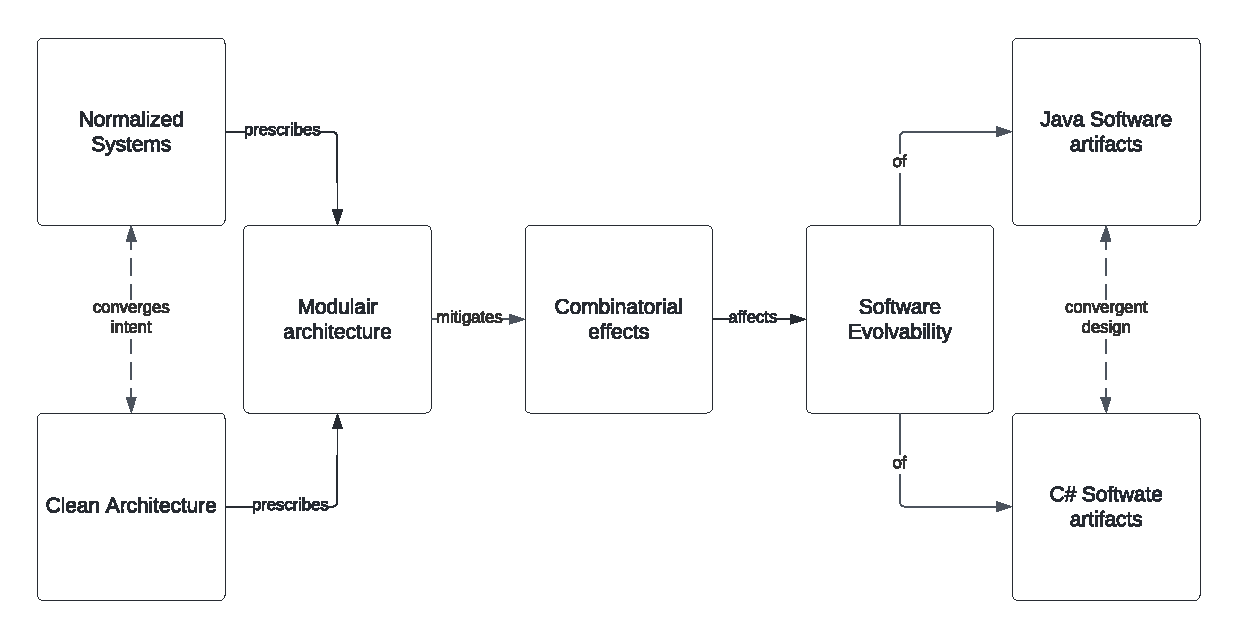
\includegraphics[width=1\textwidth]{Figures/hypothesis.pdf}
    \caption[The hypothesis graphically.]{The hypothesis graphically.}
    \label{fig:hypothesis}
\end{figure}
\section{Problem statement} \label{problem_statement} 

Since the introduction of Normalized Systems Theorems, Java EE (Java Enterprise Edition)
was used as a programming language in scientific research settings to describe the
evolvability of software architectures based on the stability concepts of systems theory
\parencite[]{mannaert_towards_2012}. \citeauthor{mannaert_towards_2012} stated in the
paper that the design theorems were formulated as modular structures that are independent
of any software language or development paradigm.

Java EE is still a prevalent programming language for enterprise- and IT organizations.
Many software solutions are created and maintained using this programming language.

\section{Conceptual framework} 
\label{conceptualframework}

Figure \ref{fig:overall_conceptual_framework} depicts the overall conceptual research
framework. It reinforces the hypothesis claim that a C\# artifact built with the
constructs from Clean Architecture can be converged with the results of Java artifacts based
Normalized Systems Theorems. 

\begin{figure}[!ht]
    \centering
    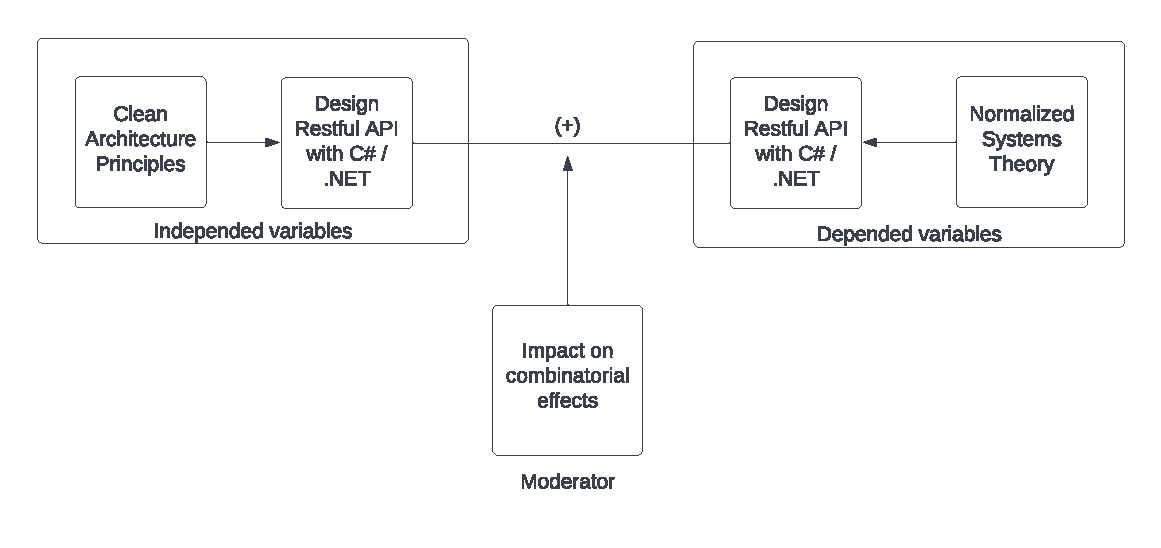
\includegraphics[width=1\textwidth]{Figures/overall_conceptual_framework}
    \caption[Overall conceptual framework]{Overall conceptual framework.}
    \label{fig:overall_conceptual_framework}
\end{figure}

\section{Research questions} \label{research_questions}
Considering the hypothesis described in \ref{conceptualframework} the following research
is determined:

\begin{center}
    \enquote*{\textit{What is the applicability of Normalized Systems Theorems
    on restful APIs designed based on the Clean Architecture principles and build with
    C\#/.NET}}
\end{center}

The following sub-questions can be formulated that support the research on the main
research question:
\begin{itemize}
    \item What is the literature stating about evolvable software systems.
    \item What is the literature stating about combinatorial effects on software changes in software systems.
    \item What is the literature stating on how one can measure combinatorial effects of a change on a software system.
    \item Which principles of Clean Architecture contribute to a reduction of
    combinatorial effects, in a way that they complement the theorems of normalized
    systems.
\end{itemize}
\chapter{Theoretical background} \label{theoreticalbackground} 


\section{Main Section 1}
\lipsum[1-1]
\section{Main Section 2}
\lipsum[1-1]
\section{Main Section 3}
\lipsum[1-1] 
% Chapter #4

\chapter{Research desgin and approach}
\chapter{Artifact design} \label{artifactdesign} 


\section{Main Section 1}
\lipsum[1-1]
\section{Main Section 2}
\lipsum[1-1]
\section{Main Section 3}
\lipsum[1-1]
\chapter{Evaluation results} \label{evaluation}


\section{Main Section 1}
\lipsum[1-1]
\section{Main Section 2}
\lipsum[1-1]
\section{Main Section 3}
\lipsum[1-1]
\chapter{Discussion} \label{discussion}


\section{Main Section 1}
\lipsum[1-1]
\section{Main Section 2}
\lipsum[1-1]
\section{Main Section 3}
\lipsum[1-1]
\chapter{Conclusies} \label{conclusions}


\section{Main Section 1}
\lipsum[1-1]
\section{Main Section 2}
\lipsum[1-1]
\section{Main Section 3}
\lipsum[1-1]

%----------------------------------------------------------------------------------------
%	THESIS CONTENT - APPENDICES
%----------------------------------------------------------------------------------------

\appendix % Cue to tell LaTeX that the following "chapters" are Appendices

% Include the appendices of the thesis as separate files from the Appendices folder
% Uncomment the lines as you write the Appendices

%% Appendix A

\chapter{Appendix 1} % Main appendix title

\label{AppendixA} % For referencing this appendix elsewhere, use \ref{AppendixA}

\section{How do I change the colors of links?}

The color of links can be changed to your liking using:

{\small\verb!\hypersetup{urlcolor=red}!}, or

{\small\verb!\hypersetup{citecolor=green}!}, or

{\small\verb!\hypersetup{allcolor=blue}!}.

\noindent If you want to completely hide the links, you can use:

{\small\verb!\hypersetup{allcolors=.}!}, or even better: 

{\small\verb!\hypersetup{hidelinks}!}.

\noindent If you want to have obvious links in the PDF but not the printed text, use:

{\small\verb!\hypersetup{colorlinks=false}!}.

%% Appendix A

\chapter{Appendix 2} % Main appendix title

\label{AppendixB} % For referencing this appendix elsewhere, use \ref{AppendixA}

\section{HSome title for an appendix?}

\lipsum[2-4]

%\include{Appendices/AppendixC}

%----------------------------------------------------------------------------------------
%	BIBLIOGRAPHY
%----------------------------------------------------------------------------------------

\printbibliography[heading=bibintoc]

%----------------------------------------------------------------------------------------

\end{document}  
